\section{Simulations}
\label{sec:srslam:simulations}

We quantitatively evaluate our approach in simulation for one soft robotic segment with a camera attached to the tip of the robot. 
We first compute trajectories that behave according to \gls{PCC} kinematics. 
Next, we render photo-realistic images for the camera attached to the tip of the segment for every time step using a virtual environment implemented in Blender. Subsequently, we process the synthetic camera images with the ORB-SLAM~\cite{mur2017orb} algorithm and projected the estimated poses of the tip of the segment into the \gls{PCC} kinematic model as outlined in Section~\ref{sec:srslam:pose_estimation}. Finally, we compare the estimated poses against the ground truth and statistically evaluate the \gls{RMSE} both for translational and rotational estimates. More details follow.

\subsection{System}\label{sub:srslam:simulations_system}
We consider a soft robotic segment of diameter \SI{20}{mm} diameter and with varying lengths $L_{0,1}$ between \SI{15}{cm} and \SI{100}{cm}.
As the camera is attached to the tip of the segment, we set $l_{\mathrm{c}_1} = L_{0,1}$ and define $T_{\check{\mathrm{c}},1}^{\mathrm{c},1} = \mathbb{I}^4$.

\subsection{Trajectories and calibration sequence}\label{sub:srslam:trajectories}
Three different trajectories are considered for the simulated movement of the soft robotic segment and its attached virtual camera. While the first one represents a planar side bending, the second one describes an “8” shape with the tip, and the last one covers a lobe of the “8”. 
Those trajectories were commanded in $\Delta_{x,1}$ and $\Delta_{y,1}$, with the following mathematical formulas:
\begin{equation}\label{eq:srslam:trajectory_parametrization}
    \Delta_{x,1} = L_{0,1} A_x \sin(2 \pi f_x) \qquad \Delta_{y,1} = L_{0,1} A_y \sin(2 \pi f_y),
\end{equation}
with $L_{0,1}$ the unextended length of the robot, $A_x$ and $A_y$ amplitudes of the sinusoids and $f_x$ and $f_y$ frequencies of the sinusoids.
The parameters $f_x$ and $f_y$ are defined as follows with $k$ representing the current time index:
\begin{equation}
    f_x = \frac{F_x (k-1)}{n_{\mathrm{t}}}, \qquad f_y = \frac{F_y (k-1)}{n_{\mathrm{t}}}.
\end{equation}
Please note that these trajectories do not contain any segment elongation. 
We list the chosen amplitudes and frequencies of the trajectories in Table~\ref{tab:srslam:trajectory_params}. Each trajectory is generated considering different robot lengths, namely \SI{15}{cm}, \SI{30}{cm} and \SI{100}{cm}. The number of time steps $n_{\mathrm{t}}$ is chosen at $120$. 
The commanding of $\Delta_{x,1}$ and $\Delta_{y,1}$ is such that the amplitude and frequency of the trajectory are independent of the number of frames (i.e., time steps).
In Figure~\ref{fig:srslam:trajectories}, we show a 3D visualization of the trajectories corresponding to a segment length of \SI{15}{cm}.

\begin{table}
\centering
\caption{Parameters of the implemented trajectories. We list the amplitudes and the frequencies of the trajectories parametrized by $\Delta_{x,1}$ and $\Delta_{y,1}$ as specified in \eqref{eq:srslam:trajectory_parametrization}.}
% \begin{scriptsize}
\begin{tabular}{lcccc}\toprule
\textbf{Trajectory} & $A_x$ & $A_y$ & $F_x$ & $F_y$\\
\midrule
Trajectory 1: planar side bending & 0.1 & 0 & 0.5 & 0\\
Trajectory 2: half 8-shape & 0.05 & 0.05 & 1 & 0.5\\
Trajectory 3: full 8-shape & 0.05 & 0.05 & 2 & 1\\
\bottomrule
\end{tabular}
% \end{scriptsize}
\label{tab:srslam:trajectory_params}
\end{table}

\begin{figure*}[ht]
  \centering
  \subfigure[Trajectory 1]{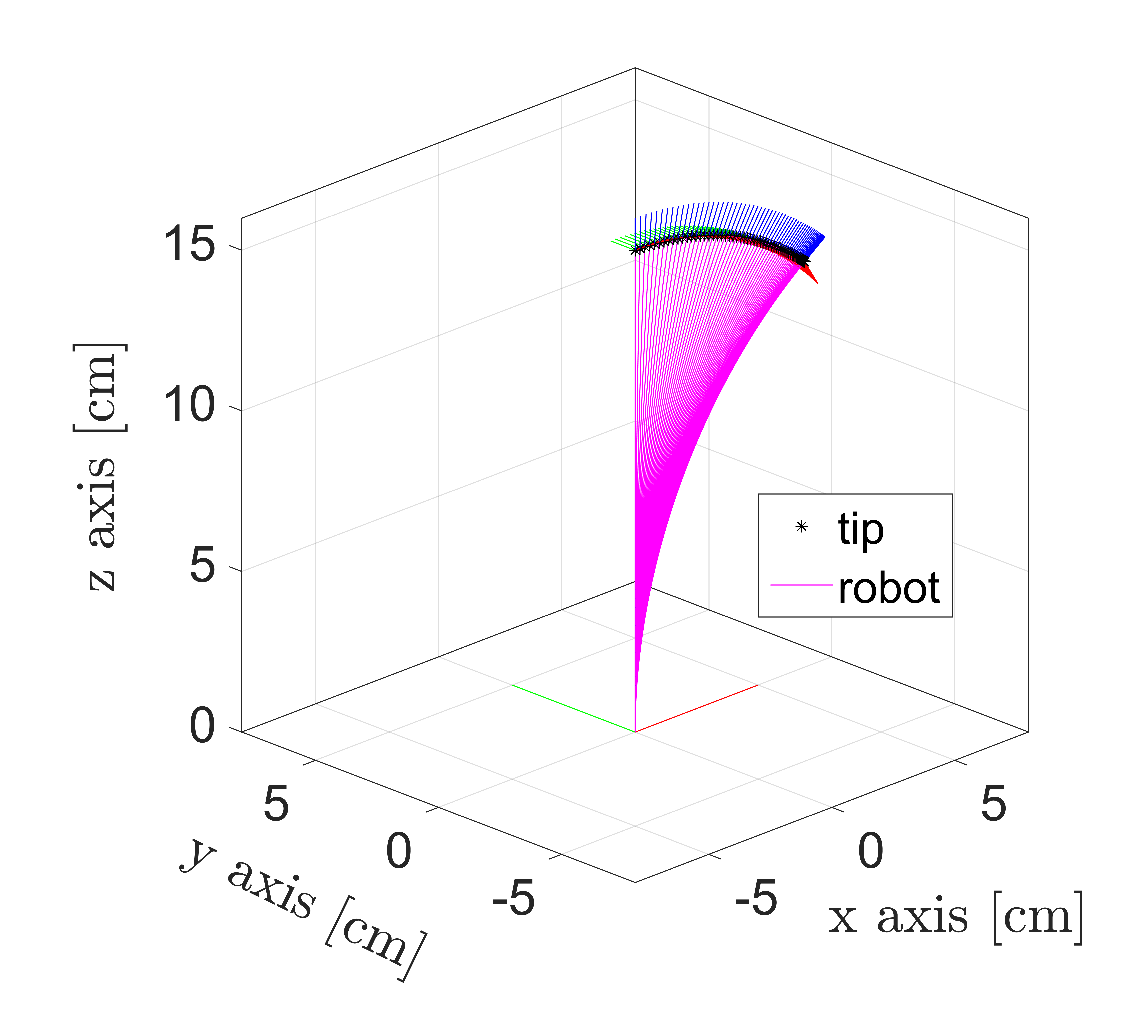
\includegraphics[width=0.21\textwidth]{srslam/figures/t1_l15_v3.0.eps}\label{fig:srslam:traj1}}
  \hspace{0.005\textwidth}% \hfill% or \hspace{5mm} or \hspace{0.3\textwidth}
  \subfigure[Trajectory 2]{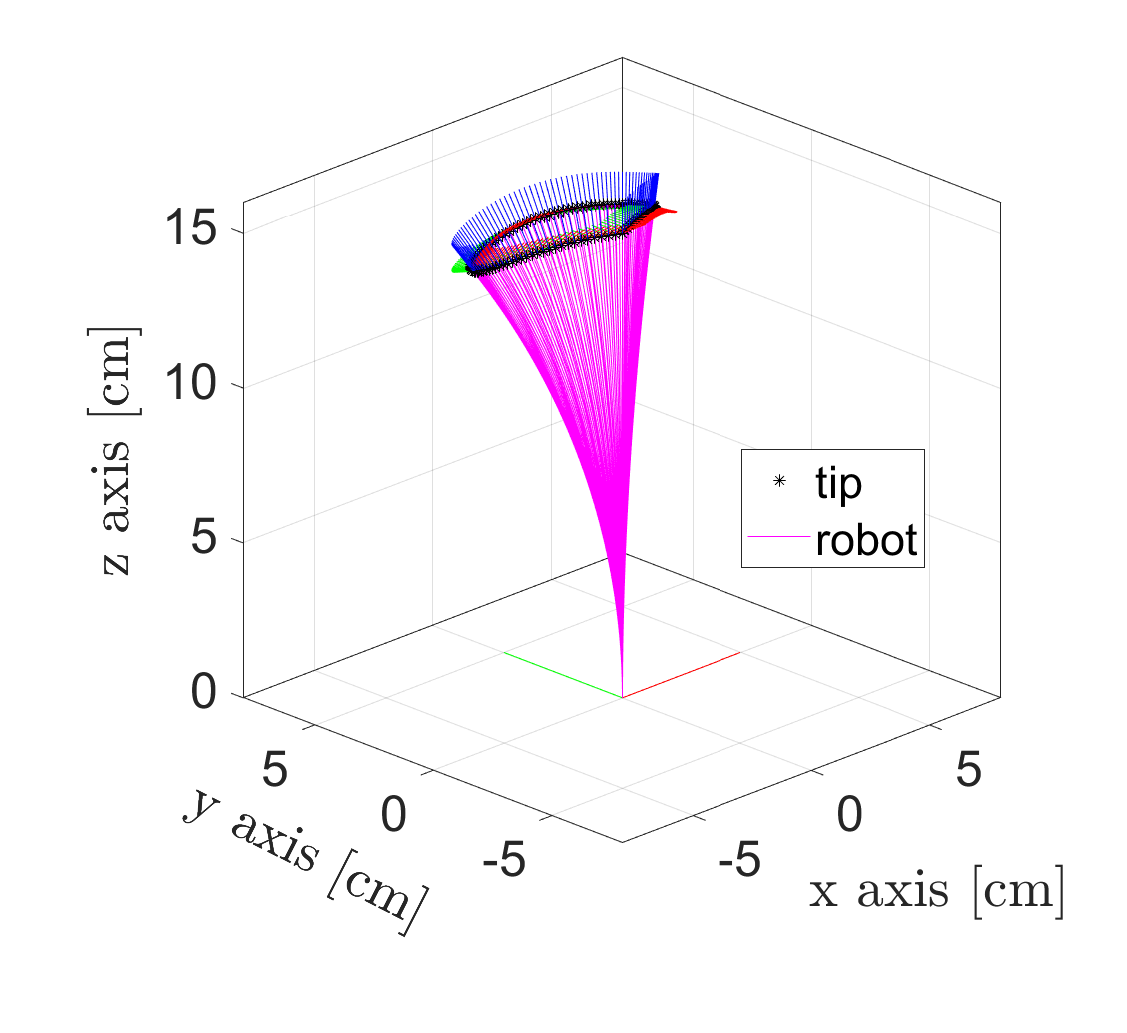
\includegraphics[width=0.21\textwidth]{srslam/figures/t2_l15_v3.2.eps}\label{fig:srslam:traj2}}\hspace{0.005\textwidth}% \hfill% or \hspace{5mm} or \hspace{0.3\textwidth}
  \subfigure[Trajectory 3]{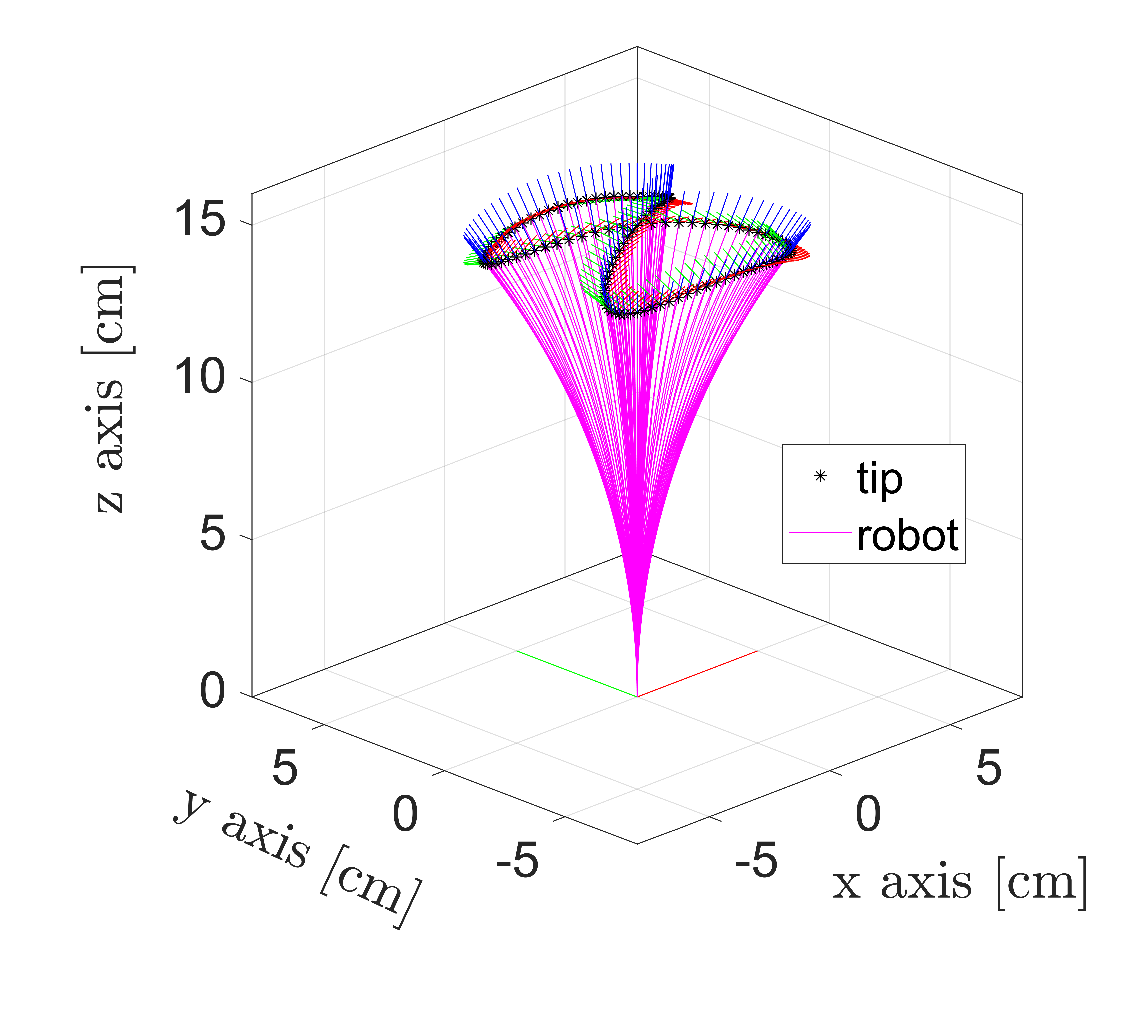
\includegraphics[width=0.21\textwidth]{srslam/figures/t3_l15_v3.1.eps}\label{fig:srslam:traj3}}\hfill
  \subfigure[Virtual interior scene]{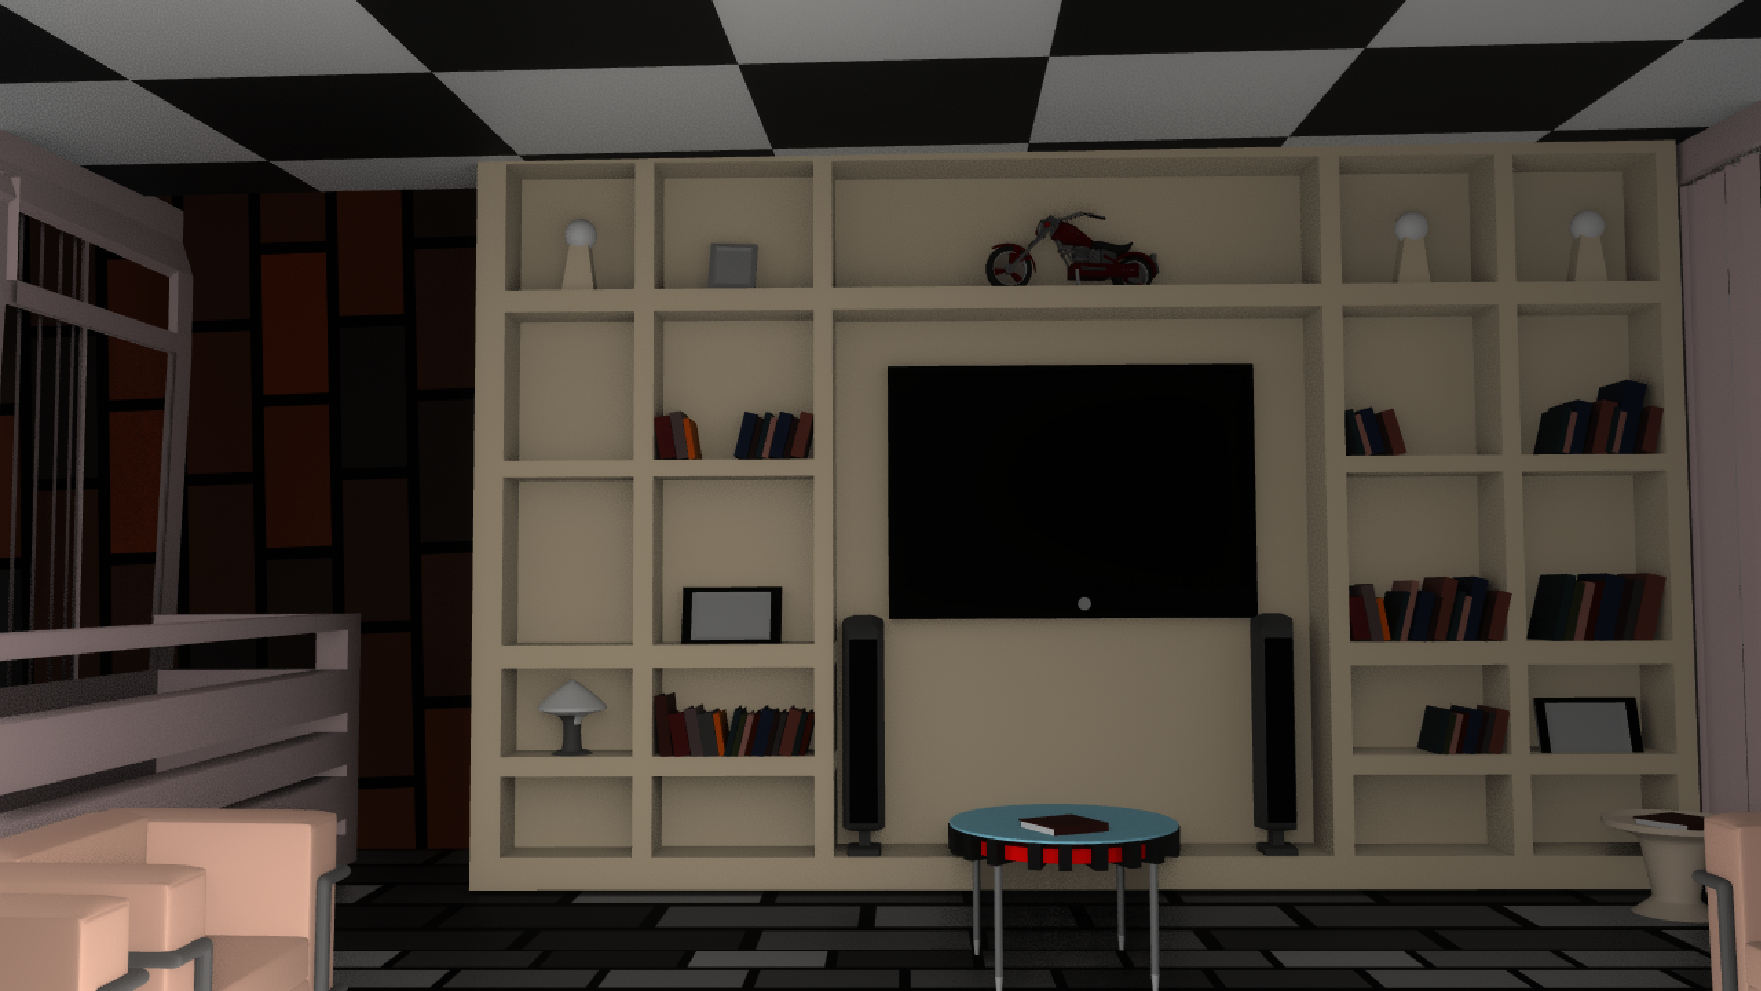
\includegraphics[width=0.3\textwidth]{srslam/figures/interior_scene.pdf}\label{fig:srslam:interior_scene}}
  \caption{3D visualization of the three trajectories used in our simulations and experiments for a segment with \SI{15}{cm} length. In magenta, we visualize the trajectory of the full robot, and in black, the tip positions. Additionally, the tip orientation (red = x-axis, green = y-axis, blue = z-axis) is displayed. The virtual interior scene used for the Blender renderings is presented in the last column.}
  \label{fig:srslam:trajectories}
\end{figure*}

In addition to the robot trajectory, a calibration sequence trajectory is designed to initialize the \gls{SLAM} map. 
It is good practice to move the camera parallel to the scene captured. Accordingly, we decide to move the camera into the $x$ cardinal direction of the segment base frame with the translation distance proportional to the robot length.

\subsection{Rendering of synthetic images}
The rendering software Blender allows us, among other things, to load a 3D model of the environment, follow customized trajectories with a virtual camera, and render photo-realistic synthetic pictures of the environment from the chosen camera perspective. We use an interior scene published by \href{https://www.nextwavemultimedia.com/html/3dblendermodel.html}{Nextwave Multimedia}. We report a view of the scene in Fig. \ref{fig:srslam:interior_scene}.
The virtual camera is set to be perspective with a focal length of \SI{30}{mm}.
For each run, we randomly initialize the trajectory at one of seven predefined launch points in the indoor environment to diversify the coverage of the environment.
The x-, y-, and z-coordinates of the seven initial positions have a standard deviation of \SI{0.5}{m}, \SI{0.2}{m}, \SI{0.4}{m} respectively. The initial orientation represented in XYZ Euler angles varies with a standard deviation of \SI{0.05}{rad}, \SI{0.13}{rad}, and \SI{1.17}{rad}.
For each trajectory, we render $120$ synthetic images along the trajectory and save them to a folder for later offline processing by the ORB-SLAM~\cite{mur2017orb} algorithm. Fig. \ref{fig:srslam:sequences_of_stills_simulations_cropped} reports a few representative stills of what the robot sees during one execution of the three trajectories discussed above.

\begin{figure*}
    \centering
    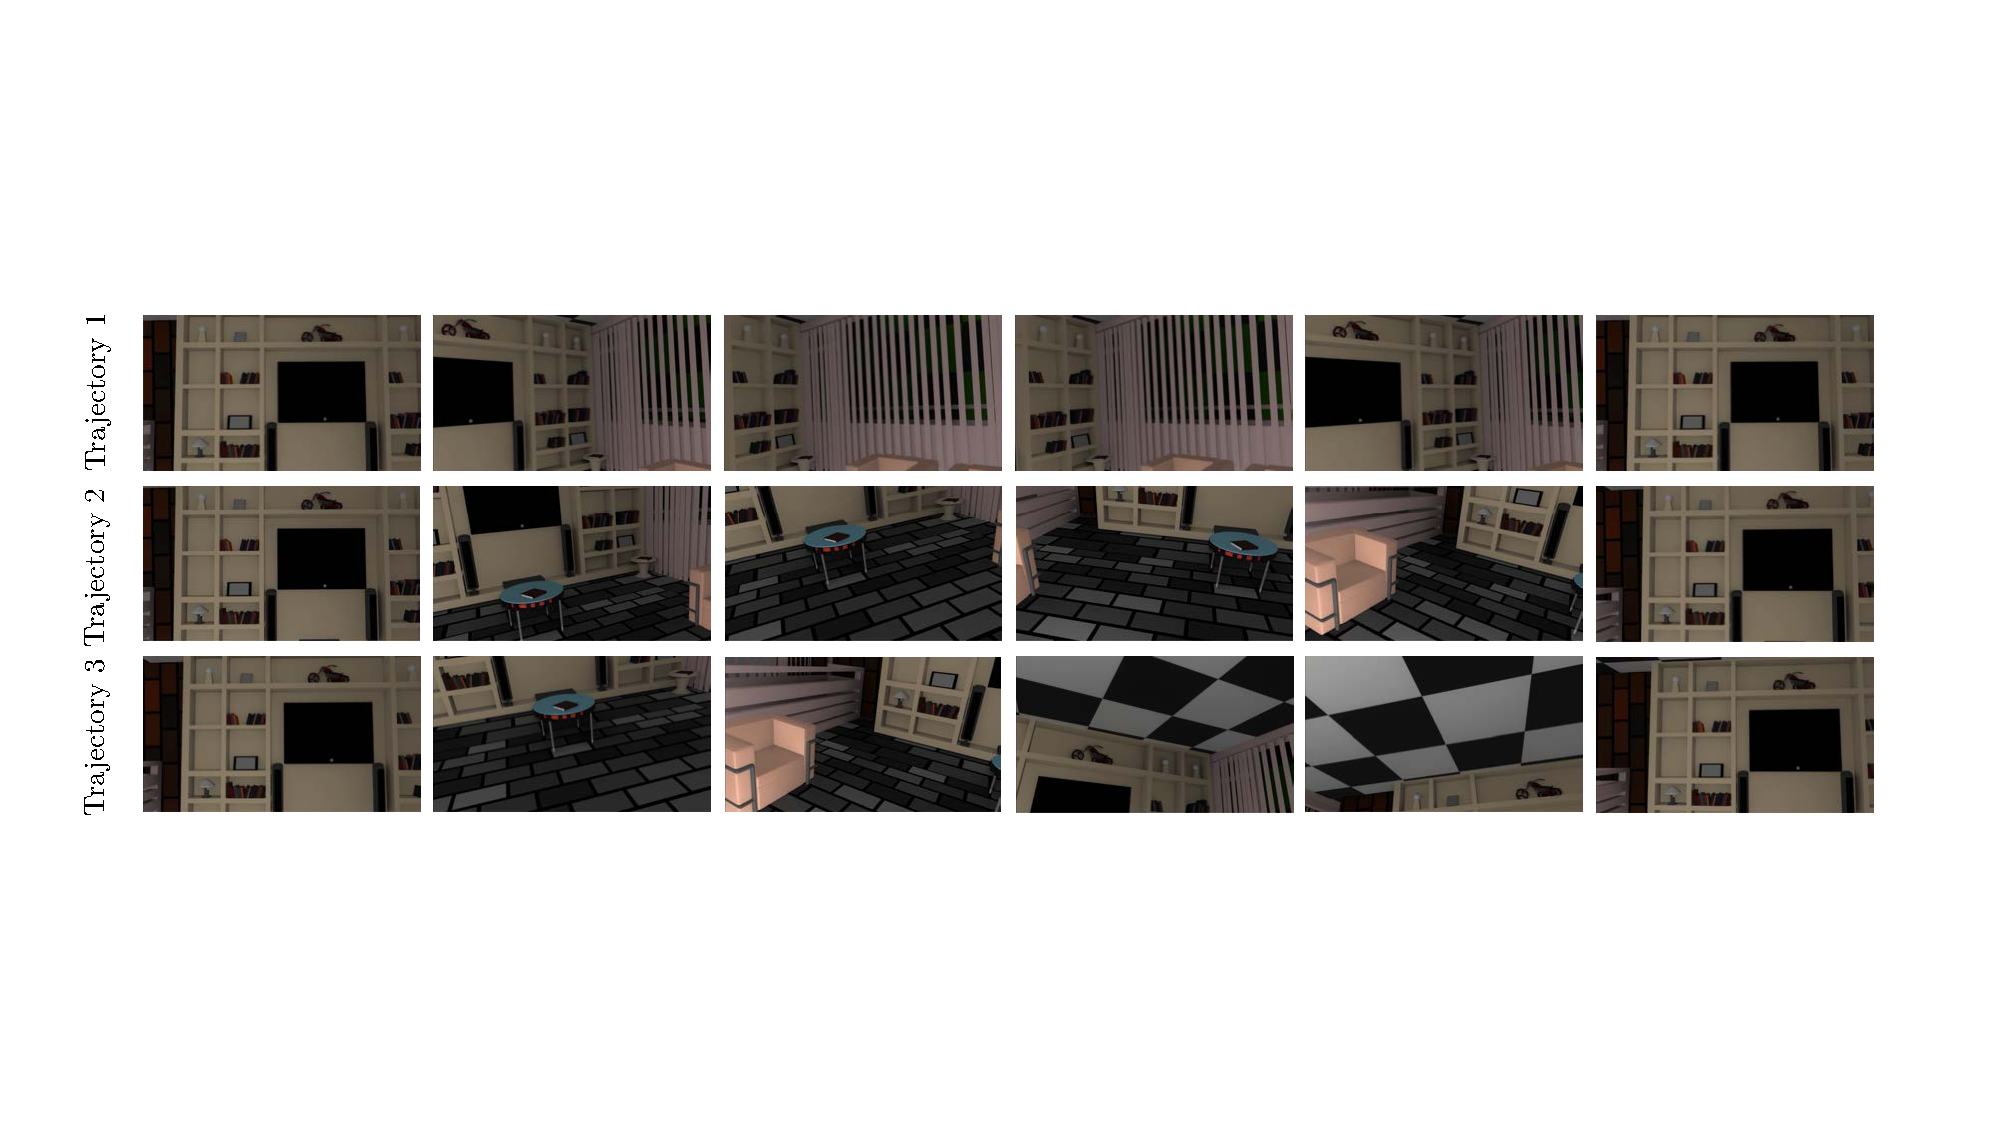
\includegraphics[width=0.9\textwidth]{srslam/figures/graphic_sequences_of_stills_simulations_compressed.pdf}
    \caption{Sequence of stills showing the rendered images by the virtual camera in Blender for three different trajectories and a robot segment of length \SI{15}{cm}. The trajectories are visualized in Figure~\ref{fig:srslam:trajectories}.}
    \label{fig:srslam:sequences_of_stills_simulations_cropped}
\end{figure*}

\subsection{Implementation of ORB-SLAM}
The synthetic images along the trajectory are processed offline by the ORB-SLAM~\cite{mur2017orb} algorithm. We rely on the official MATLAB implementation of ORB-SLAM. While we run our simulations offline to decouple any delays by the rendering and/or \gls{SLAM} pipeline, we would like to point out that other ORB-SLAM implementations, such as, for example, in C++, are able to be run in real-time at frame rates of between \SI{10}{Hz} to \SI{30}{Hz}~\cite{mur2017orb}.

\subsection{Projection into PCC kinematics}
The trade-off parameter $\lambda_\mathrm{R}$ between the rotational and the translational error in the cost function \eqref{eq:srslam:cost_fun} was manually tuned and set to $\lambda_\mathrm{R}=0.4$.
As the simulations do not contain any elongations of the segment, we set $\delta L_1 = 0$ in \eqref{eq:srslam:transformation_improved_pcc}. 
We solve the optimization problem outlined in \eqref{eq:srslam:cost_fun} using nonlinear least-squares with the Levenberg-Marquardt solver~\cite{levenberg1944method, marquardt1963algorithm} implemented in MATLAB as \emph{lsqnonlin}.

\subsection{Evaluation metrics}
To quantitatively evaluate the performance of our proposed approach, we introduce error metrics for both the translation and orientation estimates.
%
We measure the translational pose prediction error with a relative \gls{RMSE} $e_\mathrm{t}$
\begin{equation}\label{eq:srslam:evaluation_translational_error}
    e_\mathrm{t} = \frac{\sqrt{\sum_{t=1}^{n_\mathrm{t}} \left (\lVert \hat{t}_{0,t}^{\mathrm{c},1} - t_{0,t}^{\mathrm{c},1} \rVert_2 \right )^2}}{\sqrt{n_\mathrm{t}} \; l_\mathrm{traj}},
\end{equation}
where $l_\mathrm{traj}$ corresponds to the length of the trajectory and $n_\mathrm{t}$ the total number of data points along the trajectory. Similarly, we leverage the Frobenius norm for the rotational error $e_\mathrm{R}$
\begin{equation}\label{eq:srslam:evaluation_rotational_error}
    e_\mathrm{R} = \sqrt{\sum_{t=1}^{n_\mathrm{t}} \frac{\left (\big\lVert \hat{R}_{0,t}^{\mathrm{c},1} - R_{0,t}^{\mathrm{c},1} \big\rVert_F \right )^2}{n_\mathrm{t}}}.
\end{equation}
As torsion can often be neglected for soft robotic arms, we state the angle error for the orientation of the local z-axis of the tip of the segment for intuitive analysis of the orientation estimates. First, the unit vector of the local z-axis $\{ o_{1} \}_{0}$ is computed in the base frame $\{ S_0 \}$
\begin{equation}
    \{ o_1 \}_0 = R_{0,t}^{1}\begin{pmatrix}0 & 0 & 1\end{pmatrix}^\mathrm{T},
    \quad
    \{ \hat{o}_1 \}_0 = \hat{R}_{0,t}^{1}\begin{pmatrix}0 & 0 & 1\end{pmatrix}^\mathrm{T},
\end{equation}
which allows us to subsequently compute the angle error between the ground-truth z-axis of the tip $\{ o_1 \}_0$ and the estimated z-axis $ \{ \hat{o}_1 \}_0$
\begin{equation}\label{eq:srslam:evaluation_angle_error}
    e_{\theta_z} = \sqrt{\sum_{t=1}^{n_\mathrm{t}} \frac{\left (\arccos \left ( \{ o_1 \}_0 \cdot \{ \hat{o}_1 \}_0 \right ) \right )^2}{n_\mathrm{t}}}.
\end{equation}

\subsection{Results}\label{sub:srslam:simulation_results}
% \begingroup
% \setlength{\tabcolsep}{2.0pt} % Default value: 6pt
% \renewcommand{\arraystretch}{1} % Default value: 1
\begin{table*}
\centering
\caption{Relative \gls{RMSE} [\%] for translations as referenced in \eqref{eq:srslam:evaluation_translational_error} of various trajectories and of robot segments with different lengths (\SI{15}{cm}, \SI{30}{cm}, \SI{100}{cm}). We state the error as $\text{mean} \pm \text{stdev} \; (\min, \max)$ and compute the statistics over seven trials from different initial poses.}
\begin{tabular}{cclll}\toprule
\textbf{Trajectory} & \textbf{Optimization} & $L_{0,1} = \SI{15}{cm}$ & $L_{0,1} = \SI{30}{cm}$ & $L_{0,1} = \SI{100}{cm}$\\
\midrule
Trajectory 1 & No & $9 \pm 3 \; (5, 12)$ & $7 \pm 3 \; (3, 13)$ & $3 \pm 2 \; (1, 7)$ \\
Trajectory 1 & Yes & $0.4 \pm 0.2 \; (0.3, 0.8)$ & $2 \pm 1 \; (0, 4)$ & $1.0 \pm 0.7 \; (0.5, 2.3)$ \\
\midrule
Trajectory 2 & No & $9 \pm 4 \; (4, 17)$ & $6 \pm 2 \; (3, 8)$ & $1.9 \pm 0.9 \; (1.0, 3.0)$ \\
Trajectory 2 & Yes & $0.7 \pm 0.7 \; (0.3, 1.8)$ & $0.7 \pm 0.4 \; (0.2, 1.2)$ & $0.6 \pm 0.3 \; (0.3, 0.9)$ \\
\midrule
Trajectory 3 & No & $6 \pm 5 \; (3, 16)$ & $2.6 \pm 0.6 \; (1.7, 3.3)$ & $6 \pm 14 \; (1, 37)$ \\
Trajectory 3 & Yes & $2 \pm 3 \; (0, 9)$ & $0.5 \pm 0.3 \; (0.1, 0.8)$ & $2 \pm 5 \; (0, 15)$ \\
\bottomrule
\end{tabular}
\label{tab:srslam:results_simulations_translation}
\end{table*}
% \endgroup

\iffalse
\begin{table*}
\centering
\caption{Absolute \gls{RMSE} [-] for rotations computed with the Frobenius norm between rotation matrices of various trajectories and of robots with various lengths as referenced in \eqref{eq:srslam:evaluation_rotational_error}. We state the error as $\text{mean} \pm \text{stdev} \; (\min, \max)$ and compute the statistics over seven trials from different initial poses.}
\begin{tabular}{cclll}\toprule
\textbf{Trajectory} & \textbf{Optimization} & $L_{0,1} = \SI{15}{cm}$ & $L_{0,1} = \SI{30}{cm}$ & $L_{0,1} = \SI{100}{cm}$\\
\midrule
    Trajectory 1 & No & $0.010 \pm 0.004 \; (0.003, 0.015)$ & $0.016 \pm 0.007 \; (0.008, 0.027)$ & $0.027 \pm 0.017 \; (0.010, 0.051)$ \\
    Trajectory 1 & Yes & $0.007 \pm 0.002 \; (0.003, 0.010)$ & $0.012 \pm 0.007 \; (0.004, 0.023)$ & $0.027 \pm 0.019 \; (0.013, 0.062)$ \\
    \midrule
    Trajectory 2 & No & $0.02 \pm 0.02 \; (0.01, 0.05)$ & $0.011 \pm 0.006 \; (0.005, 0.022)$ & $0.015 \pm 0.008 \; (0.006, 0.025)$ \\
    Trajectory 2 & Yes & $0.02 \pm 0.02 \; (0.00, 0.06)$ & $0.016 \pm 0.009 \; (0.003, 0.025)$ & $0.019 \pm 0.008 \; (0.009, 0.030)$ \\
    \midrule
    Trajectory 3 & No & $0.1 \pm 0.2 \; (0.0, 0.4)$ & $0.010 \pm 0.002 \; (0.006, 0.012)$ & $0.2 \pm 0.4 \; (0.0, 1.1)$ \\
    Trajectory 3 & Yes & $0.1 \pm 0.2 \; (0.0, 0.4)$ & $0.02 \pm 0.01 \; (0.00, 0.034)$ & $0.2 \pm 0.3 \; (0.0, 0.9)$ \\
\bottomrule
\end{tabular}
\label{tab:srslam:results_simulations_rotation_frobenius}
\end{table*}

\begin{table*}
\centering
\caption{Absolute \gls{RMSE} [rad] for rotations computed with dot product \textcolor{red}{...}. We state the error as $\text{mean} \pm \text{stdev} \; (\min, \max)$ and compute the statistics over seven trials from different initial poses.}
\begin{tabular}{cclll}\toprule
\textbf{Trajectory} & \textbf{Optimization} & $L_{0,1} = \SI{15}{cm}$ & $L_{0,1} = \SI{30}{cm}$ & $L_{0,1} = \SI{100}{cm}$\\
\midrule
    Trajectory 1 & No & $0.005 \pm 0.002 \; (0.002, 0.007)$ & $0.009 \pm 0.005 \; (0.004, 0.018)$ & $0.02 \pm 0.01 \; (0.01, 0.04)$ \\
    Trajectory 1 & Yes & $0.005 \pm 0.002 \; (0.002, 0.006)$ & $0.008 \pm 0.005 \; (0.003, 0.016)$ & $0.02 \pm 0.01 \; (0.01, 0.04)$ \\
    \midrule
    Trajectory 2 & No & $0.02 \pm 0.02 \; (0.00, 0.04)$ & $0.006 \pm 0.002 \; (0.003, 0.010)$ & $0.009 \pm 0.005 \; (0.003, 0.016)$ \\
    Trajectory 2 & Yes & $0.01 \pm 0.02 \; (0.00, 0.04)$ & $0.005 \pm 0.002 \; (0.002, 0.009)$ & $0.013 \pm 0.006 \; (0.006, 0.020)$ \\
    \midrule
    Trajectory 3 & No & $0.1 \pm 0.1 \; (0.0, 0.3)$ & $0.006 \pm 0.001 \; (0.004, 0.007)$ & $0.1 \pm 0.2 \; (0.0, 0.4)$ \\
    Trajectory 3 & Yes & $0.1 \pm 0.1 \; (0.0, 0.3)$ & $0.005 \pm 0.002 \; (0.002, 0.008)$ & $0.1 \pm 0.2 \; (0.0, 0.7)$ \\
\bottomrule
\end{tabular}
\label{tab:srslam:results_simulations_rotation_z_angle}
\end{table*}
\fi

\begin{table*}\scriptsize
\centering
\caption{Rotational errors of various trajectories and for robot segments with different lengths (\SI{15}{cm}, \SI{30}{cm}, \SI{100}{cm}). We report both an absolute \gls{RMSE} computed with the Frobenius norm between the rotation matrices as stated in \eqref{eq:srslam:evaluation_rotational_error} and an angle error [rad] for the orientation of the z-axis of the tip of the segment as defined in \eqref{eq:srslam:evaluation_angle_error}. We state the error as $\text{mean} \pm \text{stdev}$ and compute the statistics over seven trials from different initial poses.}
\begin{tabular}{cc cc cc cc}
\toprule
    \multirow{2}{*}{\textbf{Trajectory}} & \multirow{2}{*}{\textbf{Optim.}} & \multicolumn{2}{c}{$L_{0,1} = \SI{15}{cm}$} & \multicolumn{2}{c}{$L_{0,1} = \SI{30}{cm}$} & \multicolumn{2}{c}{$L_{0,1} = \SI{100}{cm}$}\\
    & & $e_\mathrm{R}$ & $e_{\theta_z}$ [rad] & $e_\mathrm{R}$ & $e_{\theta_z}$ [rad] & $e_\mathrm{R}$ & $e_{\theta_z}$ [rad]\\
\midrule
    Trajectory 1 & No & $0.010 \pm 0.004$ & $0.005 \pm 0.002$ & $0.016 \pm 0.007$ & $0.009 \pm 0.005$ & $0.027 \pm 0.017$ & $0.02 \pm 0.01$ \\
    Trajectory 1 & Yes & $0.007 \pm 0.002$ & $0.005 \pm 0.002$ & $0.012 \pm 0.007$ & $0.008 \pm 0.005$ & $0.027 \pm 0.019$ & $0.02 \pm 0.01$ \\
    \midrule
    Trajectory 2 & No & $0.02 \pm 0.02$ & $0.01 \pm 0.02$ & $0.011 \pm 0.006$ & $0.006 \pm 0.002$ & $0.015 \pm 0.008$ &  $0.009 \pm 0.005$ \\
    Trajectory 2 & Yes & $0.02 \pm 0.02$ & $0.01 \pm 0.02$ & $0.016 \pm 0.009$ & $0.005 \pm 0.002$ & $0.019 \pm 0.008$ & $0.013 \pm 0.006$\\
    \midrule
    Trajectory 3 & No & $0.1 \pm 0.2$ &  $0.1 \pm 0.1$ & $0.010 \pm 0.002$ & $0.006 \pm 0.001$ & $0.2 \pm 0.4$ & $0.1 \pm 0.2$\\
    Trajectory 3 & Yes & $0.1 \pm 0.2$ & $0.1 \pm 0.1$ & $0.02 \pm 0.01$ & $0.005 \pm 0.002$ & $0.2 \pm 0.3$ & $0.1 \pm 0.2$\\
\bottomrule
\end{tabular}
\label{tab:srslam:results_simulations_rotation}
\end{table*}

We evaluate our proposed method in simulation on three different robot segment lengths (\SI{15}{cm}, \SI{30}{cm}, and \SI{100}{cm}) and for the three trajectories previously described. 
We state statistical results such as mean, standard deviation, and lower and upper bounds over seven separate trials, each covering a different part of the indoor environment. 
The errors are reported both for the \gls{SLAM} estimates \emph{before} optimization and \emph{after} projection into the \gls{PCC} kinematics.
While the results for the relative \gls{RMSE} of translation estimates through the entire trajectory are shown in Table~\ref{tab:srslam:results_simulations_translation}, the absolute \gls{RMSE} of rotation matrices computed with the Frobenius norm of the rotation matrices or the z-axis orientation axis angle error are displayed in Table~\ref{tab:srslam:results_simulations_rotation}.

Our results show translation errors of in average \SI{6}{\percent} to \SI{9}{\percent} for short segments and \SI{2}{\percent} to \SI{6}{\percent} \gls{RMSE} relative to the trajectory length for long segments before optimization. 
The projection into \gls{PCC} kinematics significantly decreases the translational error by between \SI{66}{\percent} and \SI{96}{\percent} to \SI{0.4}{\percent} to \SI{2}{\percent} for short segments and \SI{0.6}{\percent} to \SI{2}{\percent} for long segments.
%
We state an absolute \gls{RMSE} for the orientation estimates of the z-axis of the tip $e_{\theta_z}$ as defined in Eq.~\ref{eq:srslam:evaluation_angle_error} of between \SI{0.005}{\radian} and \SI{0.1}{\radian} after optimization.
The rotational error of the orientation estimates varies by trial but, on average, stays constant across the optimization. 
Choosing a bigger weight $\lambda_\mathrm{R}$ on the rotational loss during the optimization resulted in larger improvements for estimation the orientation at the cost of higher translational errors.